\documentclass{beamer}
\usepackage{graphicx}
\usepackage{tabularx}
\usepackage{listings}
\usepackage{xcolor}

% Theme and color scheme
\usetheme{Madrid}
\usecolortheme{seahorse}
\setbeamertemplate{itemize items}[square]

% Fix outline gray text issue - ensure black text in all contexts
\setbeamercolor{section in head/foot}{fg=black,bg=white}
\setbeamercolor{subsection in head/foot}{fg=black,bg=white}
\setbeamercolor{section in toc}{fg=black}
\setbeamercolor{subsection in toc}{fg=black}
\setbeamercolor{normal text}{fg=black}
\setbeamercolor{item}{fg=black}
\setbeamercolor{subitem}{fg=black}
\setbeamercolor{alerted text}{fg=black}
\setbeamercolor{block title}{fg=black}
\setbeamercolor{title in head/foot}{fg=black}

% Title page information
\title{Multi-Frame Story Generation System}
\subtitle{MULTI IMAGE GENERATION - Task 1: Story}
\author{Keyu HU \quad Siqi CHEN \quad Zhenzhuo LI}
\date{\today}

\begin{document}

% 1. Title Page
\frame{\titlepage}

% 2. Table of Contents
\begin{frame}{Outline}
    \tableofcontents[currentsection]
\end{frame}

% 3. Pipeline Overview
\section{PIPELINE}
\begin{frame}{PIPELINE: From Text to Multi-Frame Images}
    \begin{center}
        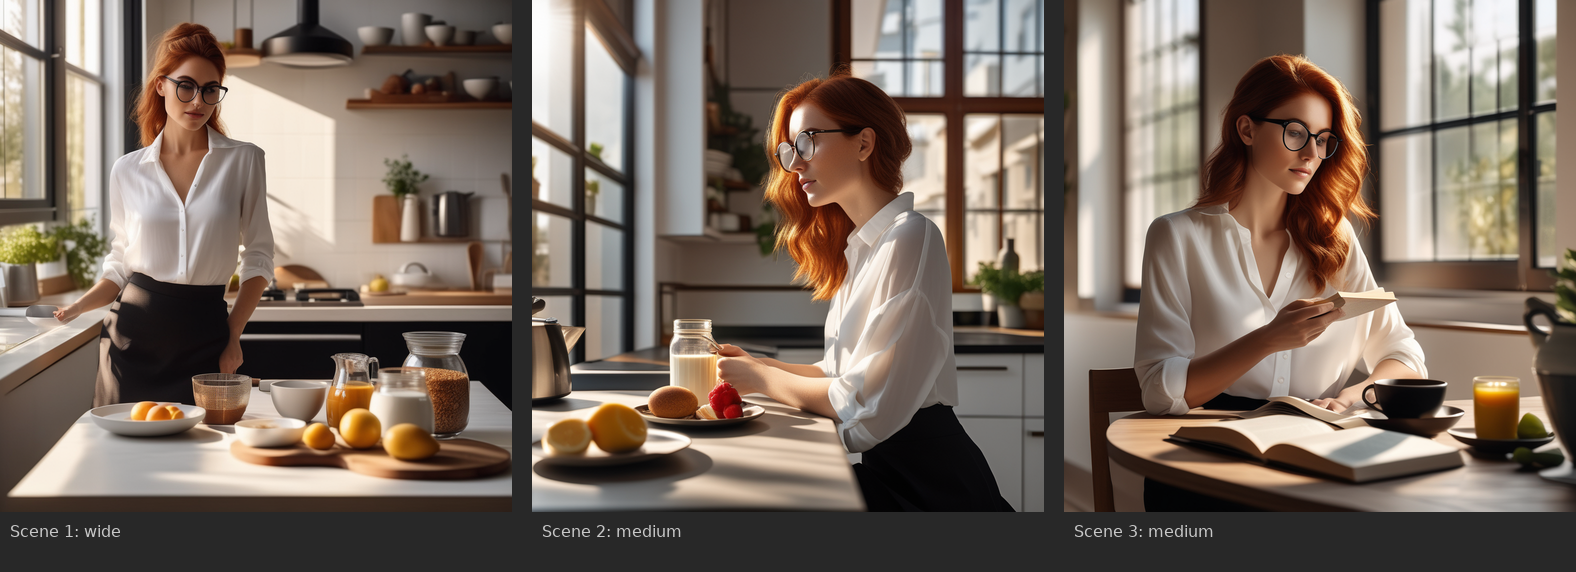
\includegraphics[width=0.85\textwidth]{images/case01_storyboard.png}
    \end{center}
    \begin{itemize}
        \item \textbf{Input}: Raw Text scripts with \texttt{[SCENE-N]} and \texttt{<Name>} tags
        \item \textbf{Processing}: LLM Processor (3-phase analysis for character/scene consistency)
        \item \textbf{Output}: JSON structure $\rightarrow$ SDXL (multi-frame image generation)
    \end{itemize}
\end{frame}

% 4. System Architecture
\begin{frame}{System Architecture}
    \begin{columns}
        \column{0.5\textwidth}
        \textbf{Four-Layer Pipeline:}
        \begin{enumerate}
            \item \textbf{Script Director} (LLM Parser)
            \item \textbf{Asset Anchor} (Character Portraits)
            \item \textbf{Core Generator} (SDXL Pipeline)
            \item \textbf{Evaluation Hub} (CLIP + LPIPS)
        \end{enumerate}
        \column{0.5\textwidth}
        \begin{block}{Key Metrics (32 test cases)}
            \begin{tabular}{lr}
                Avg CLIP Score & 0.288 \\
                Avg Consistency & 0.386 \\
                Success Rate & 100\% \\
            \end{tabular}
        \end{block}
    \end{columns}
\end{frame}

% 5. LLM Processor - Three Phases
\section{LLM PROCESSOR}
\subsection{Phase 1: Story Analysis}
\begin{frame}{Phase 1: Story Analysis}
    \begin{itemize}
        \item Character identification and unique ID assignment (e.g., \texttt{[Lily\_001]})
        \item Visual anchor extraction: clothing, hairstyle, color scheme
        \item Action decomposition per frame (e.g., ``stands by window'' $\rightarrow$ pose + environment)
    \end{itemize}
    \begin{block}{Example: Case 01 - Lily}
        \texttt{visual\_description: ``Young woman with auburn hair and round glasses, wearing a white blouse and black skirt.''}
    \end{block}
\end{frame}

\subsection{Phase 2: Prompt Generation}
\begin{frame}{Phase 2: Prompt Generation}
    \begin{itemize}
        \item Generate detailed SDXL prompts based on Phase 1 analysis
        \item Enforce cross-frame appearance consistency
        \item Multi-character scenes: LEFT/RIGHT spatial positioning
    \end{itemize}
    \begin{block}{Enhanced Prompt Structure}
        \texttt{[character\_token], [visual\_description], [action], [setting], [lighting], photorealistic, realistic photography, sharp focus, 8k detailed}
    \end{block}
\end{frame}

\subsection{Phase 3: Refinement}
\begin{frame}{Phase 3: Refinement}
    \begin{itemize}
        \item Consistency verification (clothing drift detection)
        \item Pronoun resolution (he/she/they $\rightarrow$ specific character)
        \item Visual description prefix matching for character deduplication
    \end{itemize}
\end{frame}

% 6. Case Studies - Success Examples
\section{CASE STUDIES}
\begin{frame}{Case 11: Olivia in Classroom (Excellent Consistency)}
    \begin{columns}
        \column{0.55\textwidth}
        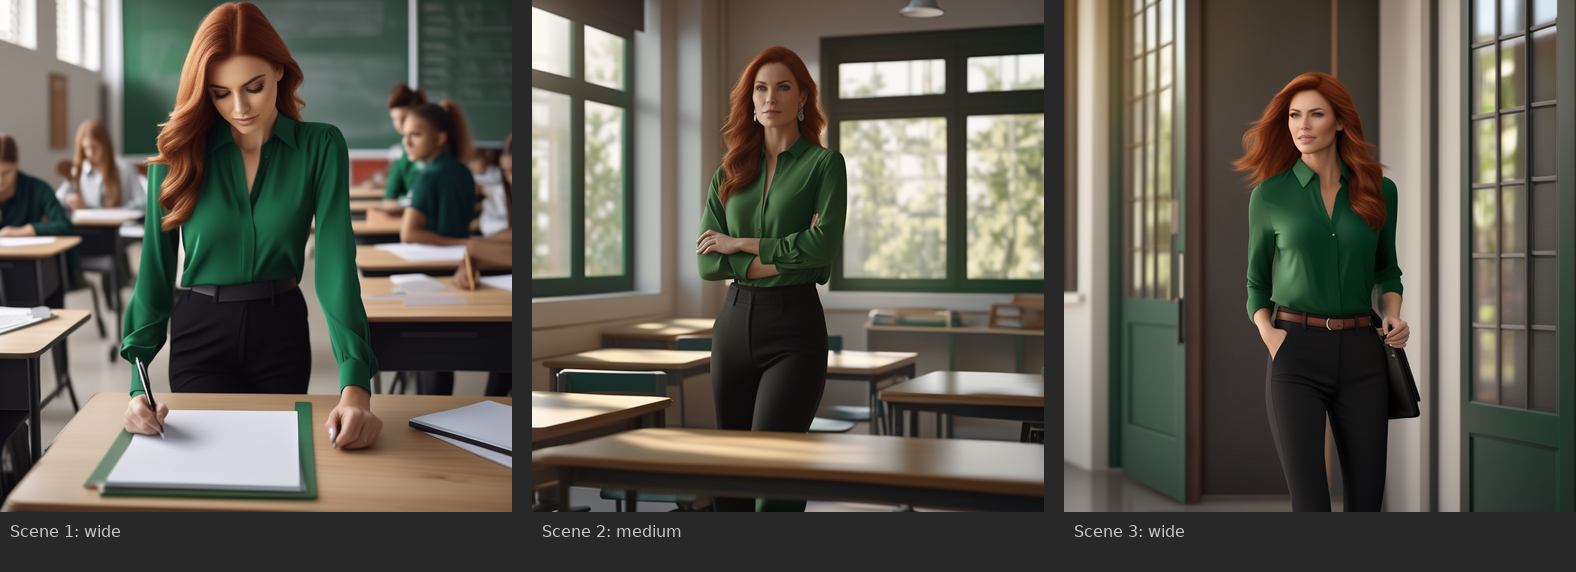
\includegraphics[width=\textwidth]{images/case11_storyboard.png}
        \column{0.45\textwidth}
        \textbf{Metrics:}
        \begin{itemize}
            \item CLIP Score: 0.331
            \item Consistency: 0.420
            \item Overall: 0.367
        \end{itemize}
        \vspace{0.5em}
        \textbf{Achievements:}
        \begin{itemize}
            \item \checkmark Auburn hair maintained
            \item \checkmark Green blouse + black pants consistent
            \item \checkmark Scene transitions smooth
        \end{itemize}
    \end{columns}
\end{frame}

\begin{frame}{Case 01: Lily Making Breakfast (Strong Facial Identity)}
    \begin{columns}
        \column{0.55\textwidth}
        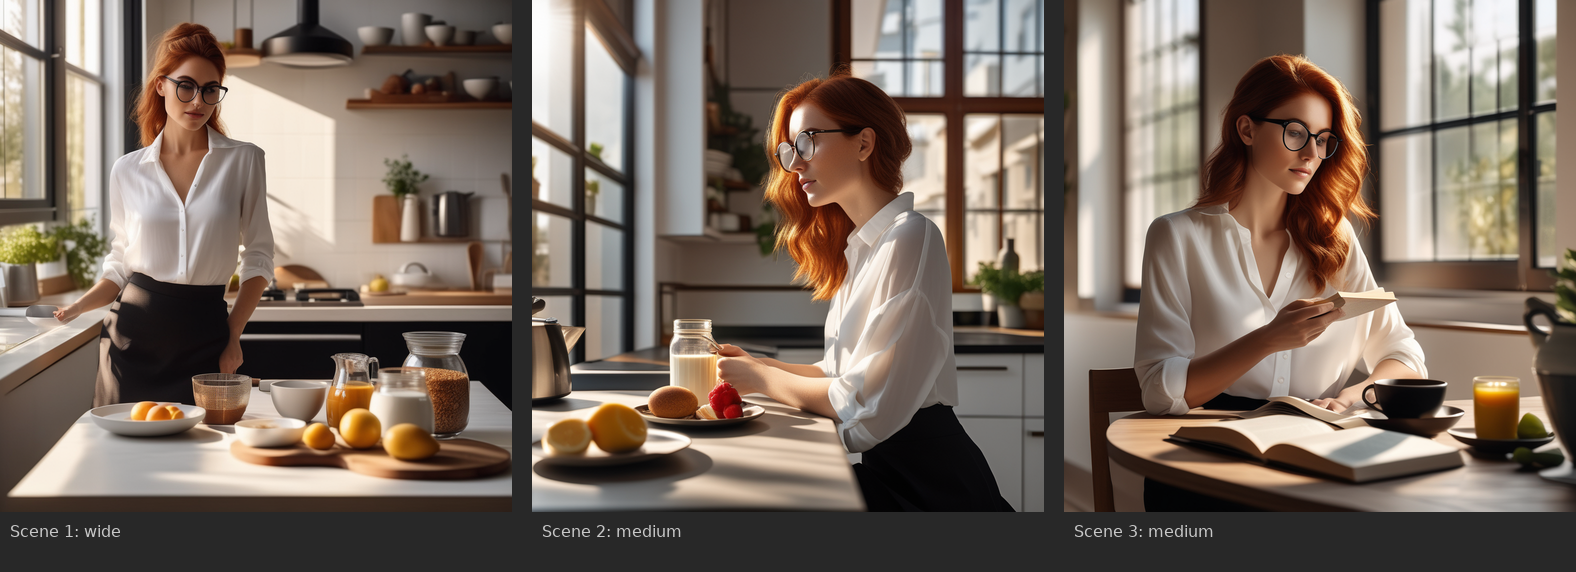
\includegraphics[width=\textwidth]{images/case01_storyboard.png}
        \column{0.45\textwidth}
        \textbf{Metrics:}
        \begin{itemize}
            \item CLIP Score: 0.310
            \item Consistency: 0.393
            \item Overall: 0.343
        \end{itemize}
        \vspace{0.5em}
        \textbf{Achievements:}
        \begin{itemize}
            \item \checkmark Round glasses preserved
            \item \checkmark Auburn hair + outfit consistent
            \item \checkmark Kitchen setting maintained
        \end{itemize}
    \end{columns}
\end{frame}

\begin{frame}{Case 12: Ethan by the Sea (Scene Coherence)}
    \begin{columns}
        \column{0.55\textwidth}
        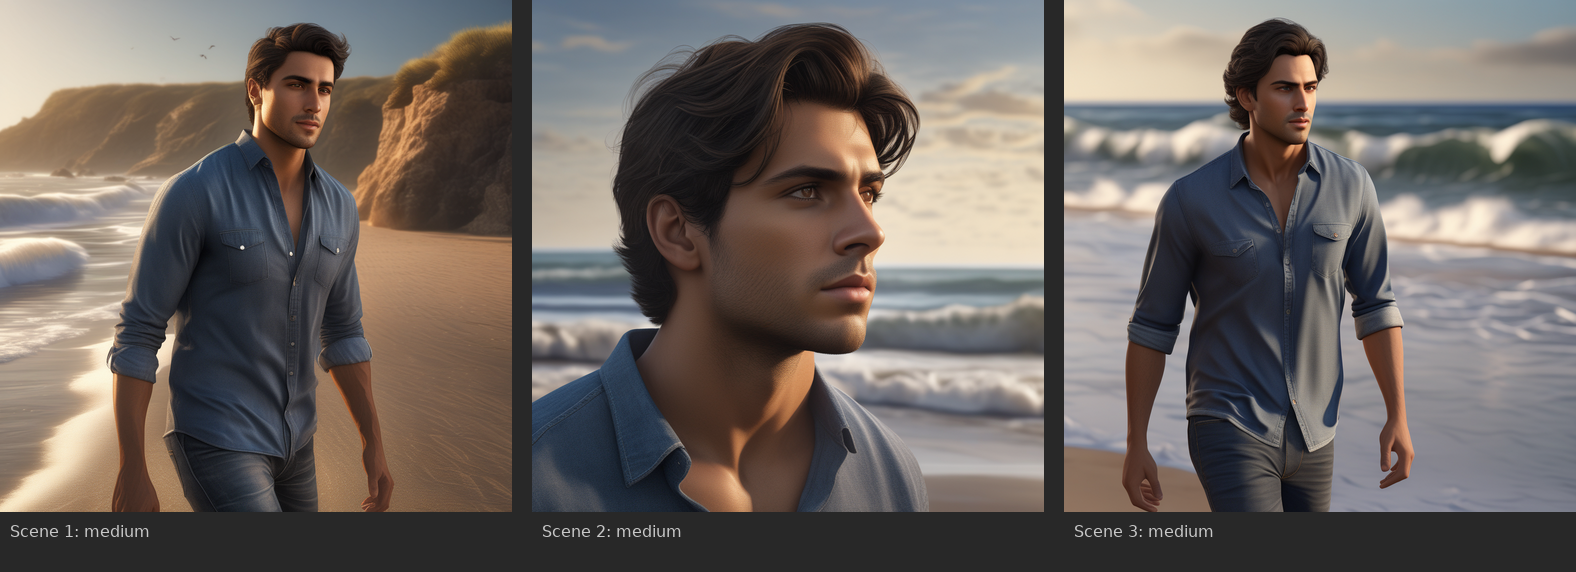
\includegraphics[width=\textwidth]{images/case12_storyboard.png}
        \column{0.45\textwidth}
        \textbf{Metrics:}
        \begin{itemize}
            \item CLIP Score: 0.288
            \item Consistency: 0.360
            \item Overall: 0.317
        \end{itemize}
        \vspace{0.5em}
        \textbf{Achievements:}
        \begin{itemize}
            \item \checkmark Beach environment consistent
            \item \checkmark Ocean lighting maintained
            \item \checkmark Walking motion coherent
        \end{itemize}
    \end{columns}
\end{frame}

\begin{frame}{Extra 02: Mark Riding Bike (Dynamic Scene)}
    \begin{columns}
        \column{0.55\textwidth}
        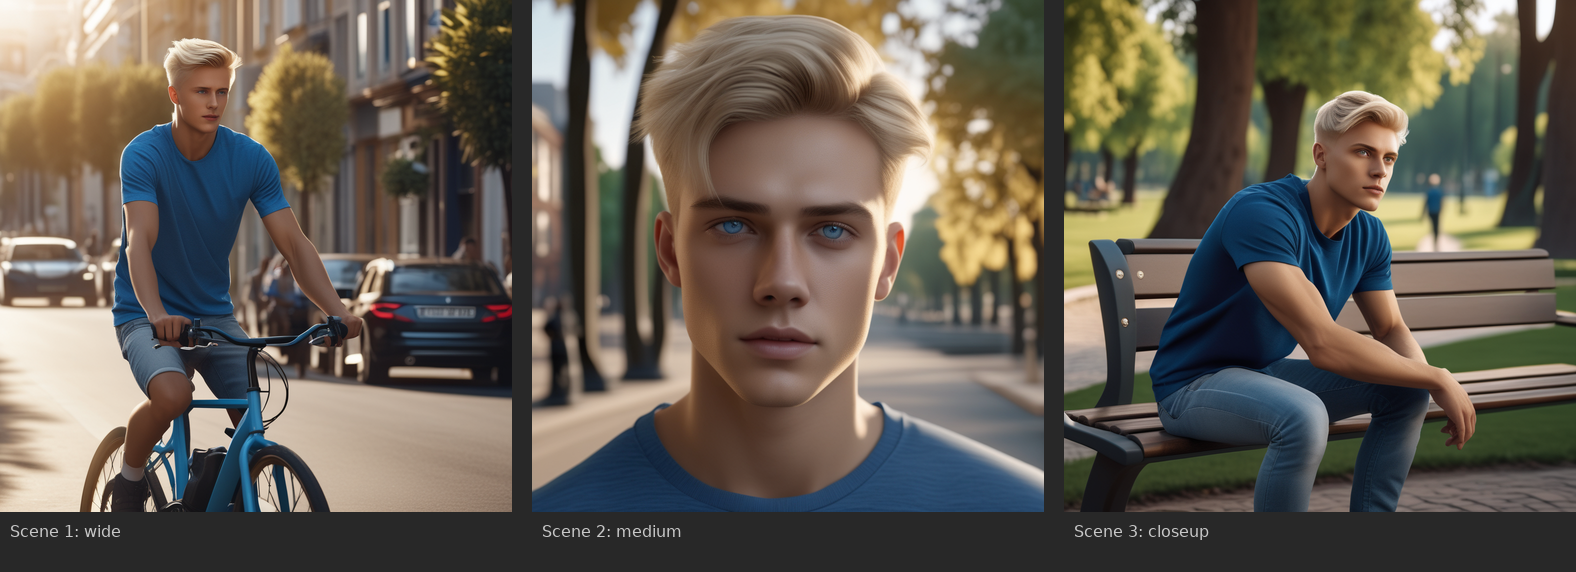
\includegraphics[width=\textwidth]{images/extra02_storyboard.png}
        \column{0.45\textwidth}
        \textbf{Metrics:}
        \begin{itemize}
            \item CLIP Score: 0.272
            \item Consistency: 0.365
            \item Overall: 0.309
        \end{itemize}
        \vspace{0.5em}
        \textbf{Achievements:}
        \begin{itemize}
            \item \checkmark Outdoor transitions smooth
            \item \checkmark Time of day consistent
            \item \checkmark Action progression clear
        \end{itemize}
    \end{columns}
\end{frame}

% 7. Challenges and Limitations
\section{LIMITATIONS}
\begin{frame}{Case 10: Baby - Animal/Non-Human Consistency Challenge}
    \begin{columns}
        \column{0.55\textwidth}
        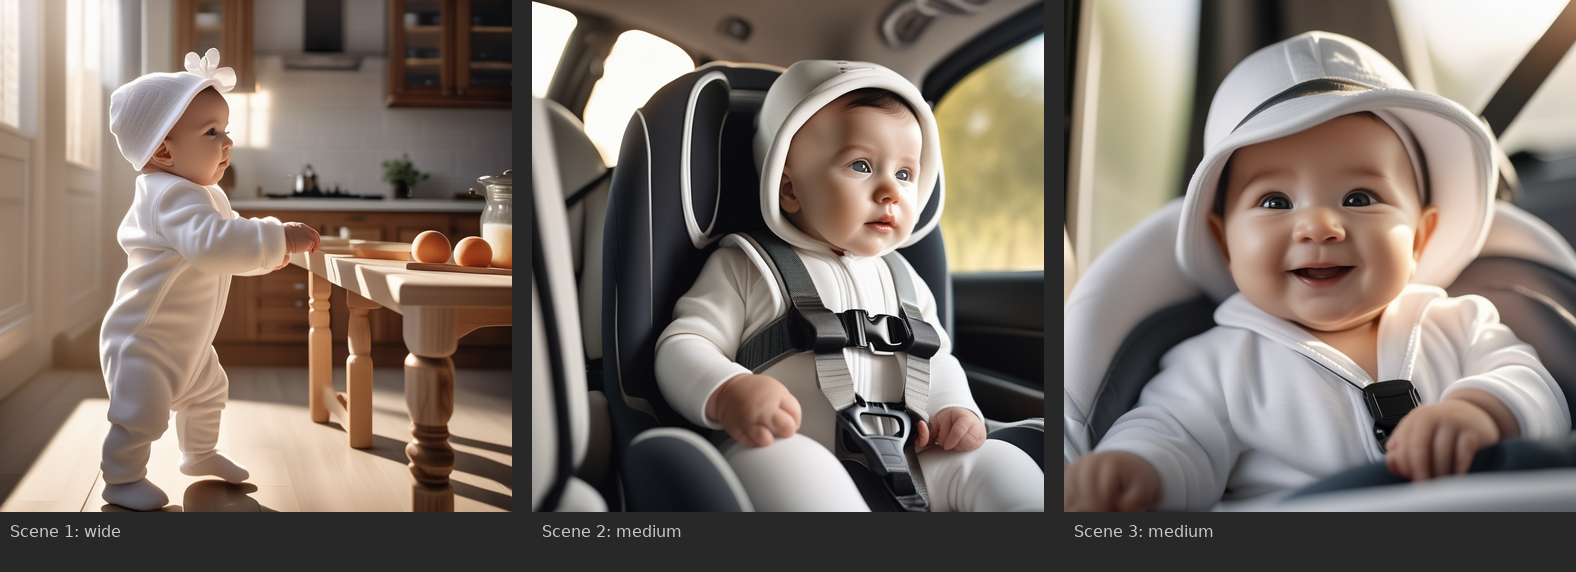
\includegraphics[width=\textwidth]{images/case10_storyboard.png}
        \column{0.45\textwidth}
        \textbf{Metrics:}
        \begin{itemize}
            \item CLIP Score: 0.294
            \item Consistency: 0.367
            \item Overall: 0.323
        \end{itemize}
        \vspace{0.5em}
        \textbf{Challenges:}
        \begin{itemize}
            \item \textbf{Inconsistent baby features}
            \item Face changes between frames
            \item Skin tone variation
        \end{itemize}
    \end{columns}
\end{frame}

\begin{frame}{Case 13: Robot - Abstract Character Misidentification}
    \begin{columns}
        \column{0.55\textwidth}
        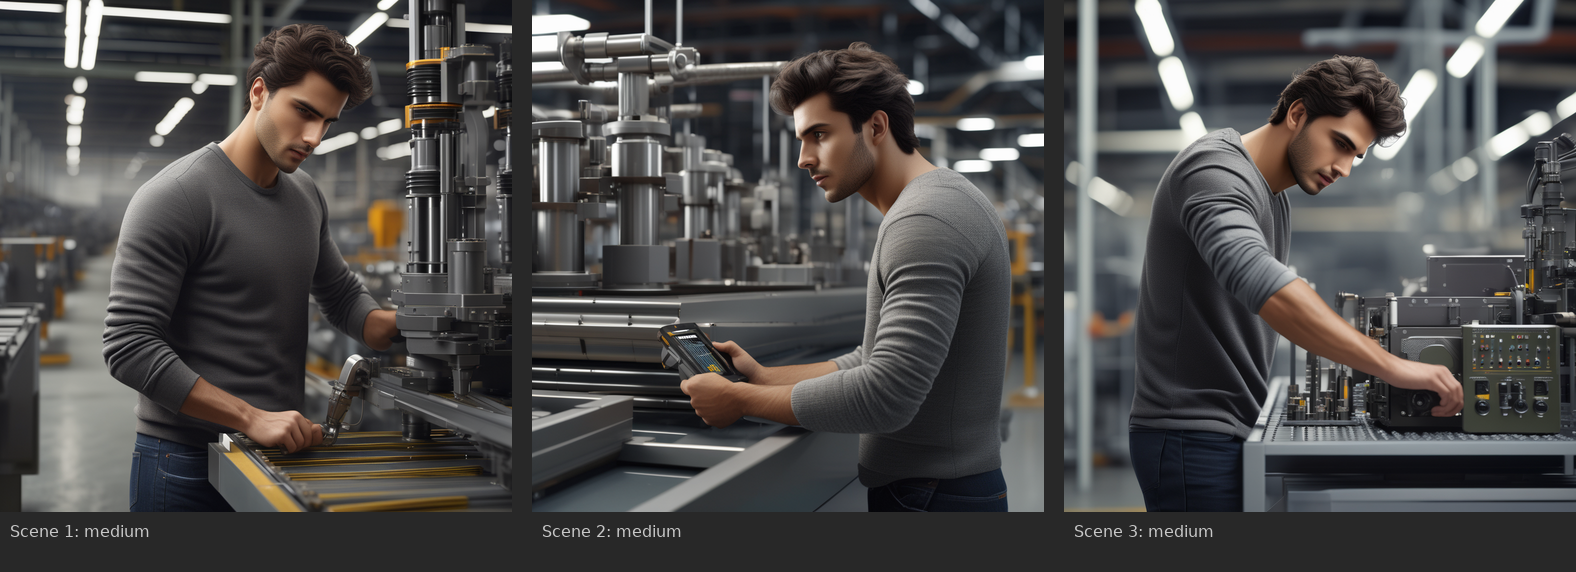
\includegraphics[width=\textwidth]{images/case13_storyboard.png}
        \column{0.45\textwidth}
        \textbf{Metrics:}
        \begin{itemize}
            \item CLIP Score: 0.205
            \item Consistency: 0.377
            \item Overall: 0.274
        \end{itemize}
        \vspace{0.5em}
        \textbf{Challenges:}
        \begin{itemize}
            \item \textbf{Robot generated as human}
            \item No metallic body features
            \item No LED lights visible
            \item Prompt override by SDXL priors
        \end{itemize}
    \end{columns}
\end{frame}

% 8. Identified Weaknesses
\begin{frame}{Summary of Limitations}
    \begin{columns}
        \column{0.5\textwidth}
        \textbf{What We Don't Achieve Well:}
        \begin{itemize}
            \item \textbf{Non-human characters}: Animals, babies show inconsistent features
            \item \textbf{Abstract entities}: Robots generated as humans
            \item \textbf{Clothing details}: Minor variations in patterns/colors
            \item \textbf{Hairstyle}: Slight changes between frames
        \end{itemize}
        \column{0.5\textwidth}
        \textbf{What We Do Well:}
        \begin{itemize}
            \item \checkmark Human facial identity
            \item \checkmark Scene/setting consistency
            \item \checkmark Lighting and mood
            \item \checkmark Story coherence
        \end{itemize}
    \end{columns}
\end{frame}

% 9. Evaluation Metrics
\section{EVALUATION}
\begin{frame}{Quantitative Results (Selected Cases)}
    \begin{table}
        \begin{tabular}{|l|c|c|c|c|}
            \hline
            \textbf{Case} & \textbf{Character} & \textbf{CLIP} & \textbf{Consistency} & \textbf{Overall} \\
            \hline
            01 & Lily & 0.310 & 0.393 & 0.343 \\
            \hline
            10 & Baby & 0.294 & 0.367 & 0.323 \\
            \hline
            11 & Olivia & 0.331 & 0.420 & 0.367 \\
            \hline
            12 & Ethan & 0.288 & 0.360 & 0.317 \\
            \hline
            13 & Robot & 0.205 & 0.377 & 0.274 \\
            \hline
            Extra 02 & Mark & 0.272 & 0.365 & 0.309 \\
            \hline
        \end{tabular}
        \caption{Metrics: CLIP Score (text-image alignment), LPIPS Consistency (inter-frame), Overall Score}
    \end{table}
\end{frame}

\begin{frame}{Metrics Explanation}
    \begin{block}{CLIP Score (Text-Image Alignment)}
        Measures how well generated images match the text prompts using OpenCLIP ViT-L-14. Target: $\geq$ 0.25
    \end{block}
    \begin{block}{LPIPS Consistency (Inter-Frame Identity)}
        Perceptual similarity between consecutive frames using learned perceptual features. Target: $\geq$ 0.30
    \end{block}
    \begin{block}{Overall Score}
        $0.6 \times \text{CLIP} + 0.4 \times \text{Consistency}$
    \end{block}
\end{frame}

% 10. Q&A
\section{Q\&A}
\begin{frame}{Questions \& Discussion}
    \begin{center}
        \LARGE Thank You! \\
        \vspace{2em}
        \large Questions?
    \end{center}
    \vspace{1em}
    \begin{block}{Key Contributions}
        \begin{itemize}
            \item LLM-driven script parsing with visual anchor extraction
            \item CLIP-based character portrait anchoring
            \item Compressed visual memory bank for consistency
            \item Quantitative evaluation pipeline (CLIP + LPIPS)
        \end{itemize}
    \end{block}
\end{frame}

% 11. Backup Slides
\section{BACKUP}
\begin{frame}{Pipeline Flow Diagram}
    \begin{center}
        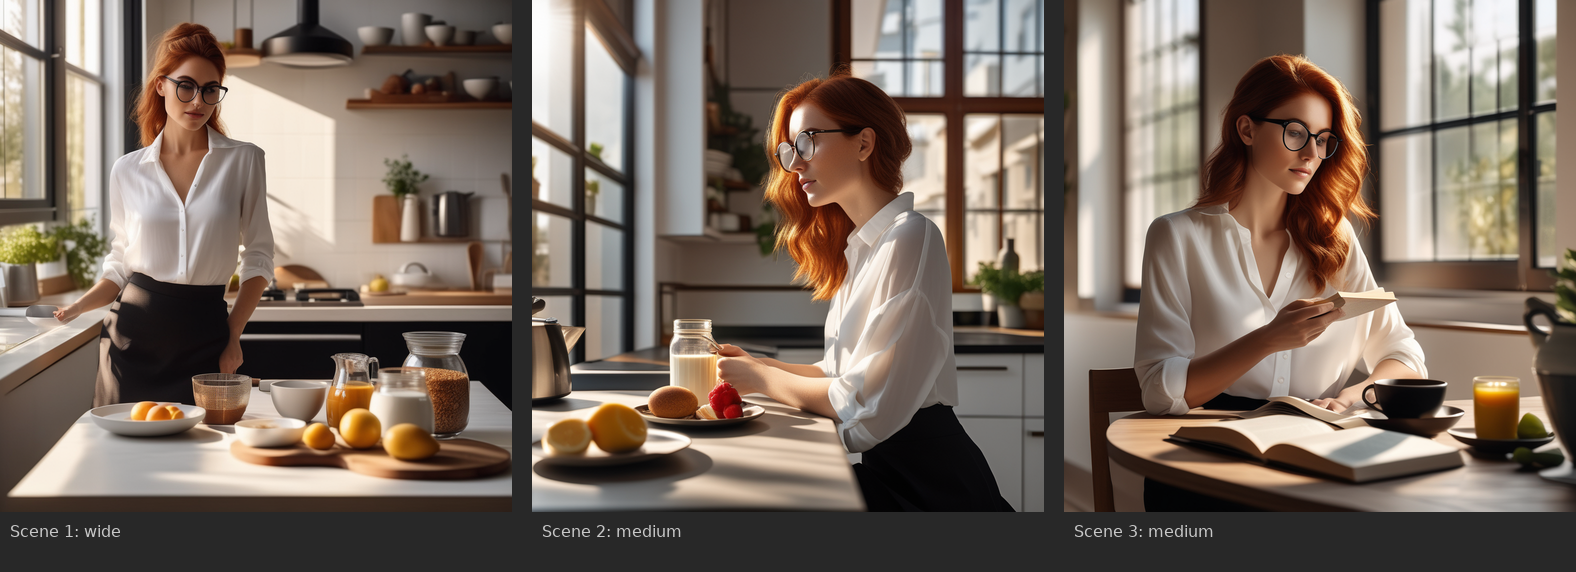
\includegraphics[width=0.7\textwidth,height=0.7\textheight]{images/case01_storyboard.png}
    \end{center}
    \begin{enumerate}
        \item Input: \texttt{[SCENE-1] <Lily> makes breakfast in the kitchen.}
        \item LLM Parser: Extract character + generate enhanced prompt
        \item SDXL Generation: 3 frames with consistent character
        \item Output: Storyboard with evaluation metrics
    \end{enumerate}
\end{frame}

\begin{frame}{Technical Details: Character Portrait Generation}
    \begin{block}{Portrait Generation Pipeline}
        \begin{enumerate}
            \item Extract visual\_description from LLM output
            \item Generate portrait using SDXL txt2img
            \item Extract CLIP features using ViT-L-14
            \item Store for cross-frame consistency
        \end{enumerate}
    \end{block}
    \begin{block}{Memory Bank}
        \begin{itemize}
            \item Compressed visual features (128-dim)
            \item Importance-weighted retrieval
            \item Temporal decay (0.9 factor)
        \end{itemize}
    \end{block}
\end{frame}

\end{document}
